% Adding a coloured vertical edge to the pages in the chapter
\ClearShipoutPicture
\AddToShipoutPicture{%
  \AtPageLowerLeft{%
    \checkoddpage
    \ifoddpage
      \begin{tikzpicture}[remember picture,overlay] % Odd page → right edge
        \draw[line width=80pt, colour_chapter7] 
             (\paperwidth,0) -- (\paperwidth,\paperheight);
      \end{tikzpicture}%
    \else
      \begin{tikzpicture}[remember picture,overlay] % Even page → left edge
        \draw[line width=80pt, colour_chapter7] 
             (0,0) -- (0,\paperheight);
      \end{tikzpicture}%
    \fi
  }%
}

%%%%%%%%%%%%%%%%%%%%%%%%%%%%%%%%%%%%%%%%%%%%%%%%%%%%%%%%%%%%%
\chapter{Towards predictions over a continuous global domain: 
global implementation of regionally-trained models}
\label{regional_to_global_training}
\graphicspath{{chapter_07/figures}{chapter_07/tables}}
%%%%%%%%%%%%%%%%%%%%%%%%%%%%%%%%%%%%%%%%%%%%%%%%%%%%%%%%%%%%%

\underline{\textbf{Authors' contribution for this chapter:}} Fatima M. Pillosu designed the study, with advice from Hannah Cloke and Christel Prudhomme, obtained the datasets, carried out the analysis, and led the writing of the manuscript. All authors assisted with writing the manuscript. Overall, 90\% of the writing was undertaken by Fatima M. Pillosu.

\vspace{\baselineskip}

\section*{PREFACE}
\addcontentsline{toc}{section}{PREFACE}

The first main analysis chapter (Chapter \ref{flash_flood_focused_verification_rainfall_based_ff}) undertakes the flash-flood-focused evaluation of short- and medium-range post-processed probabilistic point-scale rainfall forecasts. Such forecasts have been shown to predict better than the raw ERA5 flash-flood-triggering localised extreme rainfall events \citep{Pillosu_2025a}. While such an improvement in the prediction of localised extreme rainfall should enable the improved detection of areas at risk of flash floods, a flash-flood-focused assessment is fundamental to determining the extent to which enhanced rainfall prediction accuracy translates into meaningful improvements in flash flood hazard identification. In this chapter, \textcolor{colour_chapter7}{research question 1 (RQ1) "Can post-processed global NWP rainfall forecasts successfully identify areas at risk of flash floods up to medium-range lead times?"} is answered. Moreover, the first research component of this thesis is addressed, i.e. \textcolor{colour_chapter5}{developing a flash-flood-focused verification framework for predictions of areas at risk of flash floods, designed to benchmark the capability of different predictive systems}. Hence, this evaluation establishes a performance benchmark against which more sophisticated modelling approaches - incorporating additional hydrological and topographical parameters - can be measured. Such comparative analysis is essential for determining whether the increased computational demands and data requirements of complex systems yield commensurate improvements in flash flood prediction accuracy, or whether simpler precipitation-based approaches provide sufficient utility for early warning applications.

\clearpage

\section*{ABSTRACT}
\addcontentsline{toc}{section}{ABSTRACT}

\clearpage



%%%%%%%%%%%%%%%%%%%%%%
\section{Introduction}

The aspiration to develop predictions of areas at risk of flash floods over a continuous global domain confronts a fundamental paradox: whilst flash floods represent one of the most devastating natural hazards globally, causing thousands of fatalities annually and disproportionately affecting vulnerable populations in data-scarce regions, the observational infrastructure necessary for traditional model development remains concentrated in a small subset of wealthy nations. Flash floods typically occur in poorly gauged catchments, which amplifies the difficulties in rainfall and discharge data collection, and the mechanisms of flash floods are still poorly understood because of this data scarcity issue. This disparity between hazard exposure and observational capacity creates an urgent need for innovative approaches that can transcend the limitations of traditional catchment-specific modelling paradigms.

The emergence of data-driven approaches in hydrology has demonstrated remarkable success in learning complex relationships between hydro-meteorological variables and flood occurrence, yet their application to flash floods at global scales remains constrained by the severe paucity of observations in flashy catchments. Flash floods typically occur within a short time and in small or medium-sized catchments (less than 100 km2), which makes it more difficult to provide quantitative predictions than for river floods. Unlike riverine flooding, where extensive gauge networks and longer response times facilitate comprehensive data collection, flash floods occur rapidly in ungauged headwater catchments, mountain regions, and urban areas where traditional monitoring infrastructure is absent or inadequate. This challenge is particularly acute in developing nations, where the combination of limited resources, challenging topography, and rapid urbanisation creates conditions of extreme vulnerability with minimal observational capacity.

Recent advances in machine learning, particularly in transfer learning and domain adaptation, offer a transformative approach to this challenge. Decision tree learning can outperform other regionalization approaches because it generates rules that optimally consider spatial proximity and physical similarity. Rather than requiring comprehensive local observations for model training, these approaches enable models to learn generalisable hydro-meteorological relationships from data-rich regions that can be transferred to data-scarce areas. The key insight underlying this approach is that whilst specific catchment characteristics may vary globally, the fundamental physical processes governing flash flood generation—the interaction between intense precipitation, antecedent soil moisture, topography, and land surface characteristics—exhibit sufficient commonality to enable knowledge transfer across regions.

However, the development of such transferable models faces a critical trade-off between spatial coverage and data density. Models trained on high-density observations from limited geographical regions may capture local flash flood dynamics with high fidelity but fail to generalise to regions with different climatic regimes, topographies, or land use patterns. Conversely, models trained on sparse global datasets may achieve broader applicability but at the cost of reduced accuracy in capturing the rapid, localised dynamics characteristic of flash flood events. The prediction reliability is affected by data uncertainties for the gauged catchments used in prediction and by uncertainties in the regionalization procedure.
This chapter addresses Research Question 3 by systematically investigating how the coverage-density trade-off influences training strategies for developing predictions of areas at risk of flash floods over a continuous global domain. Building upon the data-driven models developed in Chapter 6, we explore three distinct approaches to training data selection: (1) random spatial sampling that maintains geographical coverage whilst reducing data density, (2) domain-restricted training that leverages high-density observations from specific regions for global application, and (3) hybrid approaches that combine limited global coverage with selective high-density regional data. Through comprehensive sensitivity analysis and evaluation across diverse hydro-climatic conditions, we aim to identify optimal strategies for balancing model transferability with predictive accuracy.

The implications of this research extend beyond methodological considerations to address fundamental questions of equity in disaster risk reduction. By demonstrating pathways for extending flash flood predictions to ungauged regions, this work contributes directly to the UN's "Early Warnings for All" initiative and the broader goal of ensuring that all populations, regardless of their location or economic status, have access to life-saving flood warnings. The insights gained from this analysis will inform the development of operational early warning systems that can bridge the gap between data-rich and data-scarce regions, ultimately saving lives and reducing the devastating impacts of flash floods globally.


%%%%%%%%%%%%%%%%%%%%%%%%%%
\section{Methods and Data}

\subsection{Training approaches}
The methodological framework examines three distinct training strategies to determine the optimal approach for developing flash flood predictions across a continuous global domain, considering heterogeneous data availability. 

\subsubsection{Training approach 1 (TA1): reduced density training}
This approach tests whether training over the full CONUS domain remains effective when flash flood observations are systematically reduced. Flash flood reports from the Storm Event Database were randomly sampled at three levels: 90\%, 50\%, and 10\% of the original dataset. The sampling was applied uniformly across the entire domain, maintaining the spatial distribution whilst reducing observation density. This approach simulates the scenario of training a global model with sparse but spatially distributed observations.

\subsubsection{Training approach 2 (TA2): domain-restricted training}
The second approach examines whether models trained on high-quality observations from limited geographical regions can effectively predict flash floods in areas where they have never observed any events. The CONUS domain was divided into four regions: East (east of 98°W), West (west of 98°W), North (north of 37°N), and South (south of 37°N). For each configuration, the model was trained using flash flood observations from only one region, with the remaining regions containing no observations during training. The trained model was then applied to predict flash floods across the entire CONUS domain. This approach directly addresses the scenario where certain parts of the world have excellent observational infrastructure whilst others have none.

\subsubsection{Training approach 3 (TA3): sparse regional coverage}
The third approach maintains training over the full CONUS domain but restricts flash flood observations to specific regions. Unlike Approach 2, the model receives hydro-meteorological data from the entire domain during training but only has access to flash flood labels in the selected region. The non-selected regions contribute only negative samples (non-flood events) to the training dataset. This configuration simulates the realistic scenario of developing a global model where flash flood reports are available only from certain countries or regions whilst meteorological data has global coverage.

\subsection{Training data configuration}
For all approaches, the baseline configuration consists of the full Storm Event Database for the CONUS from 2016-2020, containing 247,953 flash flood reports. The hydro-meteorological features remain consistent with those developed in Chapter 6, including ERA5-ecPoint rainfall, ERA5 soil moisture, and static topographic variables. Each training configuration maintains the same temporal split, with 2016-2018 for training and 2019-2020 for testing.
The spatial divisions for Approaches 2 and 3 were selected to create regions with varying flash flood characteristics. The eastern region encompasses areas with frequent convective storms and urban flash flooding, the western region includes mountainous terrain with orographic effects, the northern region experiences both snowmelt-influenced and convective events, whilst the southern region is dominated by tropical moisture and intense convective systems.

\subsection{Model configuration}
The analysis employs the XGBoost model developed in Chapter \ref{data_driven_flash_floods_short_medium_range}, applying it to systematically modified training datasets to quantify the trade-offs between spatial coverage and observation density.
The XGBoost model parameters remain consistent with those optimised in Chapter \ref{data_driven_flash_floods_short_medium_range} to ensure that performance differences arise solely from training data modifications rather than model architecture changes. The hyper-parameter values for the XGBoost model considered in this chapter are presented in Table \ref{}. No additional regularisation or modification was applied to maintain comparability across approaches.

\subsection{Performance evaluation}
Model performance was evaluated using two primary metrics. The first metric analyses the \textit{distribution of predicted probabilities} obtained with the three different training approaches to assess how different training configurations affect the model's confidence in its predictions. For this scope, violin plots will be used as changes in distribution shape, spread, and the presence of intermediate probability values provide insights into model behaviour under different data availability scenarios. The second metric considers the \textit{flash flood detection capability}, which is quantified as the number of grid cells where the predicted flash flood probability exceeds the climatological average. 

\subsection{Global Application}
Following the sensitivity analysis, the best-performing approach was selected for global application. The regionally-trained CONUS model was applied to global ERA5 and ERA5-ecPoint fields to generate predictions of areas at risk of flash floods worldwide. Due to the absence of comprehensive global flash flood databases with sufficient density for quantitative verification, the global application was evaluated through case study analysis of major flash flood events reported in international media.


%%%%%%%%%%%%%%%%%
\section{Results}

\subsection{Extension of regional training to global application}

\begin{figure}[htbp]
\centering
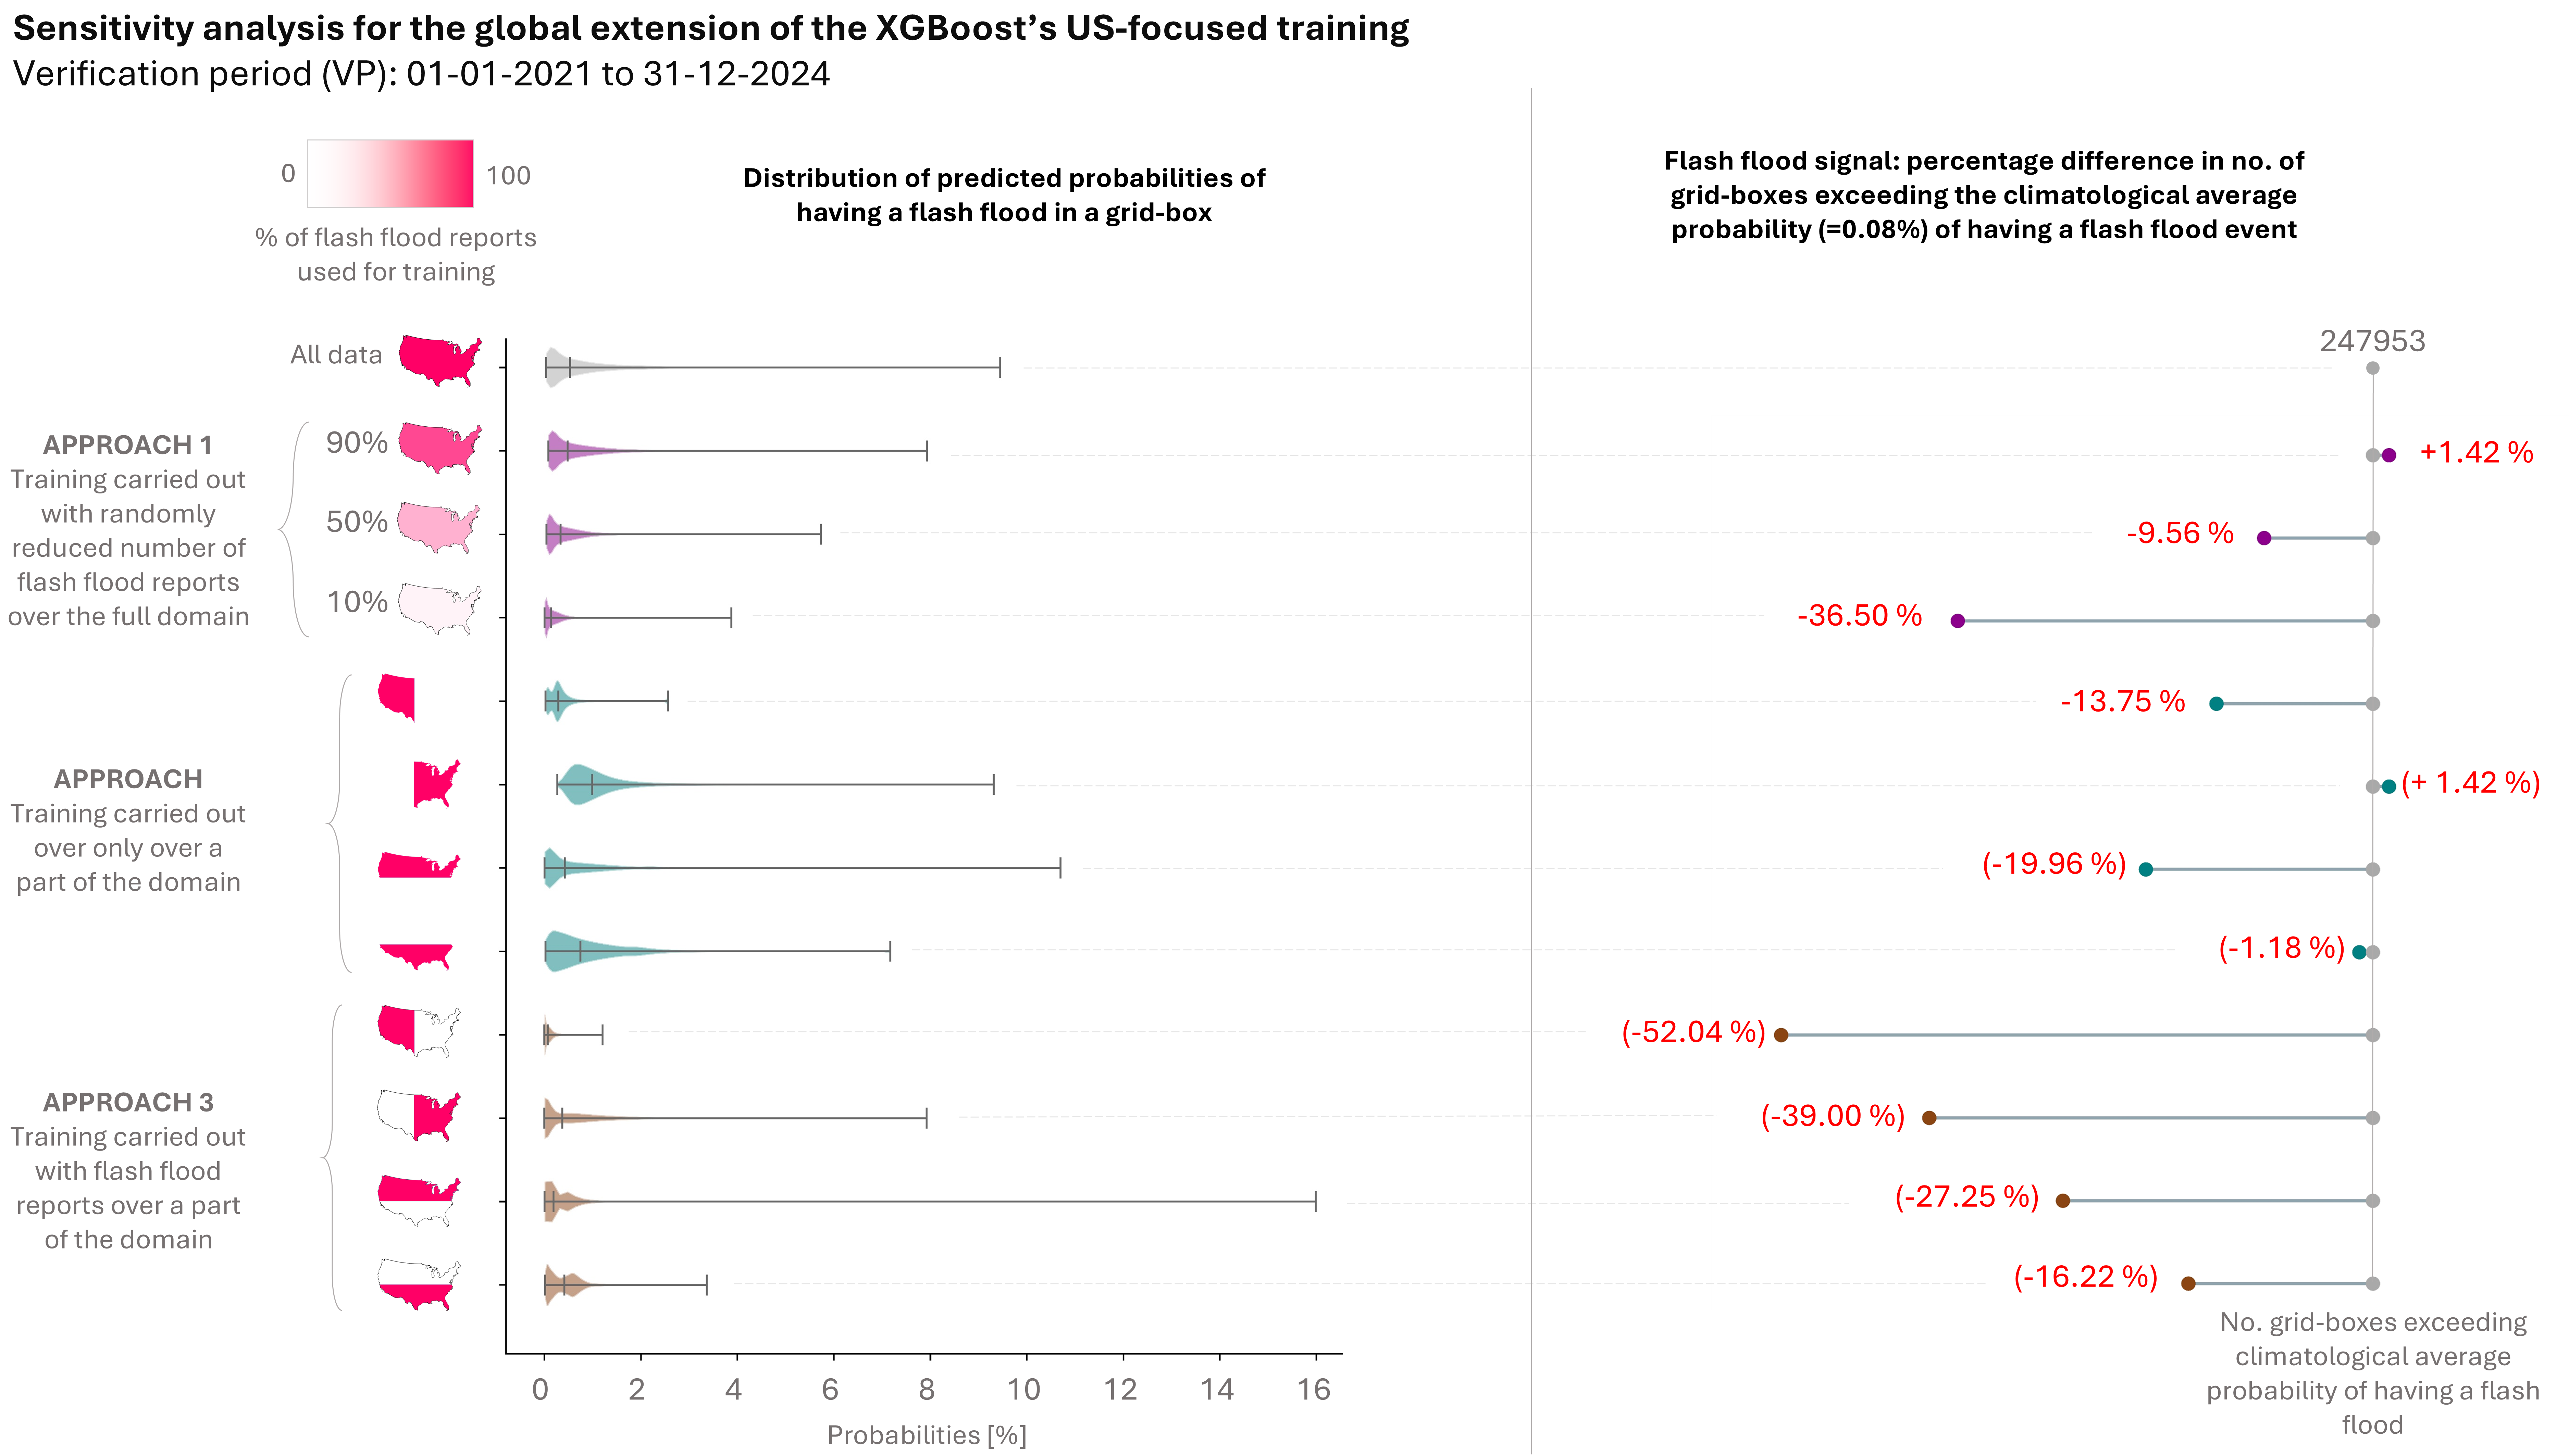
\includegraphics[width=\textwidth]{sensitivity_analysis_global_extension.png}
\caption{\textbf{Global extension performance of regionally-trained XGBoost under different U.S. training data sampling strategies.} Violin plots show predicted probability distributions, whilst dots indicate percentage change in flash flood detection capability relative to climatological baseline. Three approaches tested: random sampling (Approach 1), domain-restricted training (Approach 2), and sub-regional training (Approach 3).}
\label{fig:sensitivity_analysis_global_extension}
\end{figure}

The global application of the regionally-trained XGBoost was evaluated through three distinct approaches, each employing different spatial sampling strategies for training data inclusion (Figure \ref{fig:sensitivity_analysis_global_extension}). The baseline configuration utilising all available flash flood reports in the Storm Event Database, within the verification period, produced a conservative probability distribution, with most predictions remaining below 10\% and 247,953 grid boxes exceeding the climatological average flash flood probability (0.08\%).

Approach 1, which implemented a random reduction of the flash flood reports to predetermined percentages (90\%, 50\%, and 10\%) uniformly, across the entire U.S. domain, demonstrated variable performance. The 90\% sampling configuration merginally increased the detection capability (i.e. number of flash flood reports exceeding the climatological average of flash flood events) by 1.42\%, while the 50\% and the 90\% reductions showed, respectively, a degradation of 9.56\% and 36.50\%, suggesting non-linear relationships between training data volumes and model performance.

Approach 2 explored a spatially-constrained training strategy where the model was trained only over a certain part of the domain where observations are available. The model did not see at all the other part of the domain, and it was applied to create predictions over the whole CONUS domain. This approach simulates a global training that considers only those areas of the world with good observations during training, but uses the model globally to create predictions over the continuous global domain. The reduction in the predicted probabilities was the smallest over the three approaches, with the biggest  reductions of -13.75\% and -19.96\% when the model was trained using the parts of the domain with the smallest number of flash flood reports i.e., the east and the north, respectively. When using the parts of the domain with the biggest number of reports, i.e., the west and the south, there was an increase of +1.42\% and a minimal reduction of -1.18\% of grid-boxes with a flash flood signal.

Approach 3 explores a similar spatially constrained training, where the model is trained over the whole CONUS but with observations only over a restricted part of the domain. This approach simulates a global training of the model over the whole global domain, and considering all available reports. This is the approach with the biggest reduction in predictive ability, with reductions ranging from -52.04\% when the east side was considered and -16.22\% when the south was considered, where training data is most geographically limited.

The varying performance across different training strategies highlights the critical importance of training data representativeness for successful global model deployment. These results show that the distribution of predicted probabilities and the predictive capabilities do change for different data reduction strategies. In all cases, the probability distributions remain highly skewed towards zero probabilities. Such high concentration near the zero value does not surprise as flash floods are rare events. However, the shape and the spread of the probability values varies greatly, with more compressed distributions (with probability values rarely exceeding 2\%) over those cases that train the model with very little training data (cases 4, 5, and 9). Such compression of the probability distribution suggests that the model becomes increasingly conservative and uncertain with less data. When training instead over regions with higher training data volumes (cases 1, 6, 8, 10, and 12), the model seems to be more willing to predict moderate-to-high probabilities. The shape of the distributions is also important. Overall, the shape does not change compared to the baseline (grey violin plot, case 0) with the training approach 1, while the shapes change for approach 2 and 3. The "bulges" in the middle of the distributions, primarily in approach 2, but also in approach 3 suggest the model learned to produce intermediate probabilities (2-6\%), indicating the model developed a more nuanced risk stratification, without losing the capability to predict larger probabilities unless the training dataset is very poor, as in case 5 and 9 represented by the west coast of the CONUS (the area with the least number of flash flood reports over the CONUS). 

The application of these three training strategies suggest that while global applications can maintain reasonable performance under certain conditions, data volumes play a crucial role in determining the transferability of regional flash flood forecasting models to global applications. Due to the presented results, approach 2 is selected for the global application of the CONUS-focused training, i.e., the regional training over the CONUS, using only the Storm Event Database, is applied to global fields to create predictions of areas at risk of flash floods over a continuous global domain. While it is not possible to run a robust verification analysis over the whole global domain due to the sparse density of global datasets like EM-DAT and DesInventar, section \ref{verif_case_study} will provide a selection of case studies over the CONUS and around the world to examine the performance of the regional and global training.


\subsection{Catalogue of flash flood events}
\label{verif_case_study}


%%%%%%%%%%%%%%%%%%%%%
\section{Discussions}


%%%%%%%%%%%%%%%%%%%%%
\section{Conclusions}